\chapter{Response Theory and Molecular Properties}\label{ch:molprop}

\begin{epigraphs}
\qitem{
White light goin' messin' up my brain

White light it's gonna drive me insane
}{
--- \textsc{The Velvet Underground}
}
\qitem{What's the frequency, Kenneth? [...]

          I never understood the frequency, uh-huh}{
          --- \textsc{R.E.M.}}
\end{epigraphs}

Response theory provides an \emph{ab initio} framework for the
formulation and computation of molecular properties and can be
considered the connection between quantum chemistry and experimental
chemistry.
The response treatment of molecular properties has its roots in
time-dependent perturbation theory\autocite{Konishi2009-zb} and has been
continually developed in quantum chemistry for the past 30
years.\autocite{Olsen1985-nr, Helgaker1992-ph, Olsen1995-pf,
Christiansen1998-pe, Norman2011-ad, Helgaker2012-cz, Pawlowski2015-sq}

Section \ref{sec:exact-response} will give a brief introduction to
response theory for isolated molecules. The concepts of
quasienergy,\autocite{Christiansen1998-pe} variational perturbation
theory\autocite{Helgaker1992-ph} and pole-and-residue
analysis of response functions\autocite{Olsen1985-nr} will be introduced.
The exposition closely follows the one by \citeauthor{Saue2002-ns}
in \noparcite[ref.][]{Saue2002-ns}.
I will explicitly derive the \acrshort{SCF} response function for a
quantum/classical polarizable Hamiltonian in Section
\ref{sec:csm-response}. The derivation will employ the
density matrix-based, \acrshort{AO} formalism introduced by
\citeauthor{Thorvaldsen2008-sg} in \noparcite[ref.][]{Thorvaldsen2008-sg}.
This formalism is suitable for the derivation of arbitrary-order
response functions and their residues, also when perturbation-dependent
basis sets are considered.\autocite{Friese2015-kb, Friese2015-bu}
\paper{V} presents the arbitrary-order derivation of the \acrshort{PCM}.

\section{Response Theory in a Nutshell}\label{sec:exact-response}

Let us consider the experimentally relevant situation where a molecular
system is subject to an external source of electromagnetic radiation,
Figure \ref{fig:OR}.
Here and in the following, "external" will be used to mean an
electromagnetic field which is "weak" when compared to the
electron--electron and electron--nuclei interactions in the molecule.

\begin{figure}[tb]
  \centering
  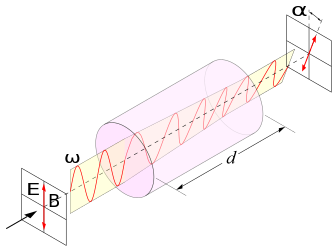
\includegraphics[width=.5\textwidth]{Optical-rotation.png}
  \caption{
  When a molecular system is subject to an external electromagnetic
  radiation of frequency $\omega$, a macroscopic, experimentally
  measurable response can be detected.
  Intensity and position of the signal can be related to the microscopic
  detail of the molecular system, as described by quantum mechanics.
  The picture depicts an optical rotation experiment where
  the linear polarization of the incident electromagnetic field
  is rotated by an angle $\alpha$ upon traversing a chiral material.
  Reproduced, with modifications, from \href{https://commons.wikimedia.org/wiki/File:Optical-rotation.svg}{Wikipedia}.
  }
  \label{fig:OR}
\end{figure}

The system can then be described by means of a combined matter--field
Hamiltonian:
\begin{equation}
  H = H_\mathrm{matter} + H_\mathrm{field} + H_\mathrm{int},
\end{equation}
where the three terms describe the molecular sample, the electromagnetic
field and their interaction, respectively.
Since our focus is on the molecular system, one can neglect the
quantized description of the field and treat the interaction term in a
semiclassical fashion.\autocite{Craig2012-zp}
The time-dependent Schr\"{o}dinger equation is now the appropriate
equation of motion:
\begin{equation}\label{eq:td-schrodinger}
  H\psi(t) = \mathrm{i}\pderiv{\psi(t)}{t},
\end{equation}
where the time-dependent, semiclassical matter--field Hamiltonian is
used:
\begin{equation}
  H = H_0 + V(t).
\end{equation}
The perturbation is a one-electron operator. We will further assume that
it is periodic in time $V(t) = V(t+T)$ and admits a discrete Fourier
decomposition:
\begin{equation}\label{eq:fourier}
  \begin{aligned}
 V(t) &=
 \sum_{k=-N}^N \expo{-\mathrm{i}\omega_k t}V(\omega_k)
 =
 \sum_{k=-N}^N\expo{-\mathrm{i}\omega_k t} \sum_X \epsilon_X(\omega_k)V_X \\
 &=
 \sum_{x}\expo{-\mathrm{i}\omega_x t}\epsilon_x V_X
  \end{aligned}
\end{equation}
where all the frequencies are integer multiples, $\omega_k=n_k \omega$
of the fundamental frequency $\omega = \frac{2\pi}{T}$.\autocite{Olsen1985-nr}
Frequencies and amplitudes in the Fourier decomposition obey the
following relations:
\begin{alignat}{2}
 \omega_{-k} = \omega_{k},
 \quad&
 \epsilon_x = \epsilon_X^*(\omega_k)
 =
 \epsilon_X(\omega_{-k}) = \epsilon^*_{-x},
\end{alignat}
since the $V(t)$ is required to be Hermitian.
For notational convenience, the perturbation operator ($X$) and
frequency ($k$) indices have been collapsed into the common index $x$.

Under the assumption that the external field is weak with respect to the
molecular field, time-dependent perturbation theory is an appropriate
tool to approximately solve Eq. \eqref{eq:td-schrodinger}.
The response theory route to molecular properties introduces a
phase-separated ansatz for the time-dependent wave function:
\begin{equation}\label{eq:phase-separated}
  \psi(t) = \expo{-\mathrm{i}F(t)}\bar{\psi}(t),
\end{equation}
where the time-derivative of the phase factor defines the time-dependent
\emph{quasienergy}:\autocite{Christiansen1998-pe, Pawlowski2015-sq}
\begin{equation}
  Q(t) = \dot{F}(t) = \Braket{\bar{\psi}(t) |
  H_0 + V(t) - \mathrm{i}\pderiv{}{t}
  | \bar{\psi}(t)}.
\end{equation}
The time-dependent quasienergy is variational, but the corresponding
time-dependent Hellmann--Feynman theorem cannot straightforwardly be
applied to the calculation of molecular properties. Fortunately, we can exploit the
periodicity of the perturbation operator to introduce the time-averaged
quasienergy:
\begin{equation}
  \aveQ =
 \frac{1}{T} \int_{-\frac{T}{2}}^{\frac{T}{2}} \diff t Q(t) =
 Q_0 + \sum_{x}\epsilon_x E_x
\end{equation}
where:
\begin{subequations}
 \begin{align}
  Q_0 &= \left\lbrace \Braket{\bar{\psi}(t) | H_0 | \bar{\psi}(t)} \right\rbrace_T
- \left\lbrace \Braket{\bar{\psi}(t) | \mathrm{i} \pderiv{}{t} | \bar{\psi}(t)}\right\rbrace_T = E_0(0) - S \\
  E_x &= \left\lbrace \Braket{\bar{\psi}(t) | V_X | \bar{\psi}(t)}\exp(-\mathrm{i}\omega_k t) \right\rbrace_T
 \end{align}
\end{subequations}
Differentiating the time-averaged quasienergy yields the time-averaged
Hellmann--Feynman theorem:
\begin{equation}\label{eq:tave-hellfeyn}
  \deriv{\aveQ}{\epsilon_X(\omega_k)}
  =
  \left\lbrace\Braket{\bar{\psi}(t) | \pderiv{H}{\epsilon_x} | \bar{\psi}(t)}\right\rbrace_T
  = E_x,
\end{equation}
which can be used to connect response functions to molecular properties.
Letting $\ket{0}$ represent the unperturbed reference state, we can
develop the Kubo expansion at zero perturbation strength of the
expectation value of the observable $H_X$:\autocite{Kubo1957-ay}
\begin{equation}
\begin{aligned}
 \Braket{\bar{\psi}(t) | V_X | \bar{\psi}(t)} &\simeq
 \Braket{0|V_X|0} +\sum_{k=-N}^N
 \response{V_X}{V(\omega_k)}{\omega_k}\expo{-\mathrm{i}\omega_k t} \\
 &+\frac{1}{2}\sum_{k,l=-N}^N
 \response{V_X}{V(\omega_k),V(\omega_l)}{\omega_k,\omega_l}\expo{-\mathrm{i}(\omega_k+\omega_l)t}
\end{aligned}
\end{equation}
response functions may be identified as the Fourier coefficients in the
expansion. These are none other but higher order derivatives of the
time-averaged quasienergy, as a comparison with the same expansion for
the right-hand side of Eq. \eqref{eq:tave-hellfeyn} will confirm:
\begin{equation}\label{eq:kubo}
\begin{aligned}
  \deriv{\aveQ}{\epsilon_x}
  &\simeq \Braket{0|V_X|0}\delta_{\omega_x} \\
  &+\sum_{y}\response{V_X}{V_Y}{\omega_y}\epsilon_y\delta_{\omega_x+\omega_y} \\
  &+\frac{1}{2}\sum_{y,z}\response{V_X}{V_Y,V_Z}{\omega_y,\omega_z}\epsilon_y\epsilon_z\delta_{\omega_x+\omega_y+\omega_z}
\end{aligned}
\end{equation}
First and higher order molecular properties can now be identified from
the response functions appearing as Fourier coefficients in the Kubo
expansion by taking the appropriate perturbation-strength derivatives at
zero field strength:
\begin{equation}\label{eq:nth-order-derivative}
  \left.\frac{\diff^n \aveQ}{\diff\epsilon_{x_1}\diff\epsilon_{x_2}\cdots\diff\epsilon_{x_n}} \right|_{\vect{\epsilon}=0}
  =
  \response{V_{X_1}}{V_{X_2}, \ldots, V_{X_n}}{\omega_{x_2},\ldots,\omega_{x_n}}\delta_{\omega_{x_1}+\cdots+\omega_{x_n}},
\end{equation}
the $\delta_{\omega_{x_1}+\cdots+\omega_{x_n}}$ notation is used to
enforce the sum rule on the probing and response frequencies involved in
the expansion:
\begin{equation}\label{eq:sum-rule}
 \sum_{i=1}^{n} \omega_{k_i} = 0
\end{equation}
Response functions quantify how, to a certain order in the perturbing
field tuples, the expectation value of a given observable is modified.
The semicolon appearing in the response functions separates the operator
$V_X$, whose response is measured, from the external perturbations
$V_Y$, $V_Z$\dots{} causing it.
From the perturbation expansion Eq. \eqref{eq:kubo}, it is clear that
permutation symmetry exists between the external perturbations provided
that the corresponding frequencies are permuted concomitantly.

Having introduced response functions as a useful tool to quantify the
effect of external perturbations on molecular properties, it is now time
to consider how to actually compute them.
In this Section, we are concerned with exact wave functions that can
thus be parametrized in a variational fashion by a set of parameters
$\vect{\lambda}$: $\ket{0}=\ket{0(\vect{\lambda})}$.
We recall that the Lagrangian method outlines in Section
\ref{sec:coupled-cluster} can be employed also in this
case.\autocite{Christiansen1998-pe, Helgaker2012-cz, Pawlowski2015-sq}
The optimal parameter set is determined upon minimization of the
time-averaged quasienergy:
\begin{equation}\label{eq:var-cond}
 \deriv{\aveQ}{\vect{\lambda}} = 0.
\end{equation}
In variational perturbation theory,\autocite{Helgaker1992-ph,
Saue2002-ns} we assume the variational parameters to be functions of the
perturbation strength parameters: $\vect{\lambda} =
\vect{\lambda}(\vect{\epsilon})$.
Furthermore, we require the stationarity condition to hold at \emph{all}
perturbation strengths, with $\lambda(0) = 0$, for convenience.

The perturbation-strength total derivative at zero perturbation strength
of the time-averaged quasi energy is:
\begin{equation}
\begin{aligned}
 \left[\prod_{i=1}^n \deriv{}{\epsilon_{x_i}}\right]\aveQ
 &= Q^{[n]}_{x_1 \ldots x_n}
 =
 Q^{[n]}_{0; x_1 \ldots x_n}
 + \sum_{j=1}^{n}E^{[n-1]}_{x_j;x_1\ldots x_{j-1}x_{j+1}\ldots x_n} \\
 &=
 \left[\prod_{i=1}^n \deriv{}{\epsilon_{x_i}}\right]Q_0
 + \sum_{j=1}^n
 \left[\prod_{i\neq j}^{n-1} \deriv{}{\epsilon_{x_i}}\right]E_{x_j}
\end{aligned}
\end{equation}
Notice that this is just an alternative and more verbose notation for
Eq. \eqref{eq:nth-order-derivative}, which allows to express response
functions in terms of wave function perturbed parameters.
Application of the chain rule to the total derivatives in fact yields:
\begin{subequations}
 \begin{align}
   Q^{[1]}_{a} &=
   \sum_{\sigma}\left[
   Q^{[1]}_{0; \sigma}\lambda^{[1]}_{\sigma;a} + E_{a}
   \right]\delta_{\omega_a} \\
   Q^{[2]}_{ab} &=
   \sum_{\sigma\tau}\left[
   \lambda^{[1]}_{\sigma;a}Q^{[2]}_{0;\sigma\tau}\lambda^{[1]}_{\tau;b}
   + Q^{[1]}_{0; \sigma}\lambda^{[2]}_{\sigma;a}
   + E^{[1]}_{a;\sigma}\lambda^{[1]}_{\sigma;b}
   + E^{[1]}_{b;\sigma}\lambda^{[1]}_{\sigma;a}
   \right]\delta_{\omega_a+\omega_b} \label{eq:linres}
 \end{align}
\end{subequations}
where the following tensors were introduced:
\begin{subequations}
 \begin{align}
 Q^{[n]}_{0; \sigma_1\cdots \sigma_n} &=
 \frac{\partial^n Q_0}{\partial\lambda_{\sigma_1}\cdots\partial\lambda_{\sigma_n}} \\
 E^{[n]}_{x;\sigma_1\cdots \sigma_n} &=
 \frac{\partial^n E_x}{\partial\lambda_{\sigma_1}\cdots\partial\lambda_{\sigma_n}} \\
\lambda^{[n]}_{\sigma;x_1\dots x_n} &=
\frac{\partial^n \lambda_\sigma}{\partial \epsilon_{x_1}\cdots\partial \epsilon_{x_n}}
 \end{align}
\end{subequations}

The response equations, determining the $\vect{\lambda}^{[n]}$ tensor of
perturbed wave function parameters, are obtained by differentiating the
variational condition on the time-averaged quasienergy Eq.
\eqref{eq:var-cond}:\autocite{Olsen1985-nr, Helgaker1992-ph, Christiansen1998-pe}
\begin{equation}
 R_{\sigma;x_1\cdots x_n}^{[n]} = \left[\prod_{i=1}^n \deriv{}{\epsilon_{x_i}}\right]
\left. \deriv{\aveQ}{\lambda_\sigma}\right|_{\vect{\epsilon}=0} = 0.
\end{equation}
The determination of second-order properties requires the knowledge of
the first-order response of the wave function:
\begin{subequations}
 \begin{align}
 R_{\sigma}^{[0]} &= Q_{0;\sigma}^{[1]} = 0 \\
 R_{\sigma;a}^{[1]} &= \sum_{\tau}Q_{0;\sigma\tau}^{[2]}\lambda_{\tau;a}^{[1]} + E_{a;\sigma}^{[1]} = 0.
 \label{eq:1st-order-response}
 \end{align}
\end{subequations}
The time-averaged quasienergy formalism allows to formulate response
properties to static and dynamic fields on an equal footing as
perturbation-strength derivatives.
Moreover, variational perturbation theory achieves a transparent
derivation of the necessary response equations.\autocite{Helgaker1992-ph}

Let us consider in more detail the form of the linear response function
Eq. \eqref{eq:linres}. The formal solution to the response equation Eq.
\eqref{eq:1st-order-response} can be obtained by inverting the
\emph{Hessian}. Eq. \eqref{eq:linres} can then be rewritten as:
\begin{equation}
  \response{V_A}{V_B}{\omega_b}
  =
   -\sum_{\sigma\tau}
   E^{[1]}_{a;\sigma}
   \left[\mat{Q}^{[2]}_{0}\right]^{-1}_{\sigma\tau}
   E^{[1]}_{b;\tau}.
\end{equation}
Expansion into the exact eigenbasis of $H_0$ yields the
\gls{SOS} expression for the linear response function:
\begin{equation}
  \response{V_A}{V_B}{\omega_b}
  =
  -\sum_{n>0}\left[
  \frac{\braket{0|V_A|n}\braket{n|V_B|0}}{\omega_{n0}-\omega_b}
  +
  \frac{\braket{0|V_B|n}\braket{n|V_A|0}}{\omega_{n0}-\omega_a}
  \right]\delta_{\omega_a+\omega_b}.
\end{equation}
The excitation energies of the system appear in the denominators
$\omega_{n0} = E_n - E_0$ and can thus be identified as the \emph{poles}
of the response function. Moreover, the \emph{residues} at
the poles are the transition moments determining the intensity of
spectroscopic transitions:
\begin{equation}
  \lim_{\omega_b\rightarrow\omega_{n0}}
  \response{V_A}{V_B}{\omega_b}
  = \braket{0|V_A|n}\braket{n|V_B|0}.
\end{equation}
A similar analysis holds also for higher order response functions. The
pole structure of the higher order quantities also conveys information
about the excited states \emph{via} single and double
residues.\autocite{Olsen1985-nr, Christiansen1998-pe, Helgaker2012-cz}

The derivation above holds for an exact state, a situation that is never
realized in common practice. The power of response theory, however, is
in its applicability to exact and approximate state theories alike.
As noted by \citeauthor{Norman2011-ad}, a response theory treatment of
molecular properties can be summarized into the following four
steps:\autocite{Norman2011-ad}
\begin{enumerate}
    \item Single out a quantity of interest that can be connected to
      molecular properties. In our case, the time-averaged
      quasienergy;
    \item Introduce a suitable parametrization of the time-dependent,
      phase-separated wave function;
    \item Devise the appropriate equation of motion, based on the
      time-dependent Schr\"{o}dinger equation, for the time-dependent
      wave function parameters;
    \item Identify response functions and response equations.
\end{enumerate}
Thus, one can formulate and compute molecular properties based on
the approximate state ans\"{a}tze of quantum chemistry.
An interesting formulation of \acrshort{SCF} response theory is the
open-ended \acrshort{AO} density matrix-based approach presented by
\citeauthor{Thorvaldsen2008-sg}.\autocite{Thorvaldsen2008-sg}
By formulating the perturbation-strenght derivative of the time-averaged
quasienergy Lagrangian in terms of the \acrshort*{AO} density matrix,
the authors were able to formulate arbitrary order response functions
in the \acrshort*{AO} basis.
The density matrix is the variational degree of freedom and response
equations can be obtained by differentiation of the \gls{TDSCF}
equation, the stationarity condition on the density matrix.
The approach lends itself to an efficient \acrshort*{AO}-based
implementation,\autocite{Larsen2000-hj, Kjaergaard2008-hy} can fully
leverage different response parameters elimination
schemes,\autocite{Thorvaldsen2008-sg, Kristensen2008-hv} and is amenable
to an open-ended, recursive implementation.\autocite{Ringholm2014-gx,
Friese2015-kb, Friese2015-bu}
We will base our derivation of \acrshort*{SCF} response theory for
quantum/classical polarizable Hamiltonians of this framework.

\section{SCF Response Theory for Quantum/Classical Polarizable Hamiltonians}\label{sec:csm-response}

The development of response theory for quantum/classical polarizable
Hamiltonians has moved almost at the same pace as the polarizable
models themselves.
An ample literature exists in the context of the
\acrshort{PCM},\autocite{Cammi1994-qj, Cammi1996-wf, Cammi1996-vx,
Cammi1999-rb, Cammi2003-qy, Frediani2005-nc, Ferrighi2010-pm}
polarizable \acrshort{MM} models,\autocite{Curutchet2009-bt, Olsen2010-wa,
Lipparini2012-hx, Lipparini2012-tl}
and general \acrshort*{QM}/\acrshort*{MM}/Continuum models.\autocite{Steindal2011-ki, Caprasecca2012-ir, Lipparini2013-ud}

Solvent relaxation is an important point when formulating response
properties. Solvation dynamics occurs on timescales and through
relaxation modes that are typical of the solvent molecular structure and of the
peculiar solute-solvent interactions.
This is clearly difficult to model with continuum models, since the
entire frequency spectrum of the permittivity $\diel(\omega)$ would be
required.\autocite{Ingrosso2003-ev, Caricato2005-lo,
Mennucci2005-vi, Caricato2006-ba, Corni2015-pe}
However, if one consider the initial steps of an electronic excitation
process, a Franck--Condon-like response of the solvent can be assumed.
Nuclear motions inside and among solvent molecules will not be able to
follow the fast rearrangement of the solute electronic density, the
corresponding part of the response will remain frozen in the state
immediately previous the change.
The polarization vector will then be (approximately) a sum of two
components:
\begin{equation}
 \vect{P} \simeq \vect{P}_\mathrm{fast} + \vect{P}_\mathrm{slow},
\end{equation}
this is equivalent to consider only the asymptotic limits of the solvent
dielectric spectrum, \ie the static $\diels$ and optical
dielectric constants $\dield$.

The variational setting introduced in Section \ref{sec:variational},
offers a series of advantages also in the formulation of response
theory. As already noted, a classical counterpart to the
Hellmann--Feynman theorem holds:
\begin{equation}\label{eq:classical-HF}
  \deriv{U_\mathrm{pol}}{F} = \pderiv{U_\mathrm{pol}}{F}
  + \pderiv{U_\mathrm{pol}}{\s}\pderiv{\s}{F}
  = \pderiv{U_\mathrm{pol}}{F},
\end{equation}
which forms the basis for our formal development in
\paper{V}.\autocite{pcm-openrsp}
There we show how the variational polarization functional can
successfully achieve a transparent derivation of arbitrary order
response functions, when the fixed-cavity approximation for the
\acrshort*{PCM} is assumed.
Here we report a summary of our findings in \paper{V} employing the
classical functional in supermatrix form in Eq. \eqref{eq:supermatrix-functional}.
In the notation of \citeauthor{Thorvaldsen2008-sg}, we introduce the
generalized free energy:
\begin{equation}\label{eq:generalized-KS-energy}
  \begin{aligned}
 \tilde{\mathcal{G}}
 &=
 \tilde{\mathcal{E}}
 + \frac{1}{2}{}^t\tilde{\p}\V\tilde{\p} +
 {}^t\tilde{\p}\Tr(\tilde{\mathbfup{s}}\pertmat{D}) \\
 &\eqtr
 \left[\pertmat{h} + \pertmat{V}^{t} +
 \frac{1}{2}\pertmat{G}^{\gamma}(\pertmat{D}) -
 \frac{\mathrm{i}}{2}\pertmat{T}\right]\pertmat{D}
 + \tilde{E}_\mathrm{xc}[\tilde{\rho}(\pertmat{D})] + h_\mathrm{nuc}
 + \frac{1}{2}{}^t\tilde{\p}\V\tilde{\p}
 + {}^t\tilde{\p}\tilde{\mathbfup{s}}\pertmat{D},
 \end{aligned}
\end{equation}
whose perturbation-strength derivatives at zero perturbation strength
will yield the desired response functions.

Due to the implicit time-dependence of $\pertmat{D}$ and
$\tilde{\sigma}$, higher-order
derivatives of the KS generalized energy will require application of the
chain rule. The ${mn, abc\ldots}$ superscript describes how and to which
extent the chain rule was applied for a given term, \ie the number of explicit
differentiations with respect to the variational densities, so that
\begin{equation}\label{eq:differential}
  \mathcal{G}^{mn, abc}
  =
  \frac{\partial^{m+n+3}\mathcal{G}}{\partial(\mat{D}^T)^m\partial\p^n\partial\epsilon_a\partial\epsilon_b\partial\epsilon_c}
  =
    \mathcal{E}^{m, abc} +
  \frac{\partial^{m+n+3}U_\mathrm{pol}}{\partial(\mat{D}^T)^m\partial\p^n\partial\epsilon_a\partial\epsilon_b\partial\epsilon_c} \text{.}
\end{equation}
In this notation, the index $m$ denotes the order of differentiation
with respect to the density matrix $\mat{D}$, while the index $n$ symbolizes
the order of differentiation with respect to the \acs{ASC} density $\sigma$.
Differentiation with respect to the density matrix will result in a
$2m$-rank tensor, while differentiation with respect to the
\acs{ASC} density will result in a function of the continuous cavity
index $\vect{s}$. For higher-order properties, mixed terms involving both density
matrix and \acs{ASC} density differentiation may generally occur.
In the \emph{fixed-cavity approximation}, the cavity is kept frozen at a
given molecular geometry.\autocite{Cammi1994-qj}
Under this simplifying assumption, only the linear interaction term in
the polarization functional eq.~\ref{eq:PCM-functional} will be affected
by the movements of the nuclei \emph{via} the dependence of basis functions on
the molecular geometry.
Its perturbation-strength derivative will then be
\begin{equation}\label{eq:PCM-derivative}
 \deriv{}{\epsilon_a}\left\lbrace
 U_\mathrm{pol}
 \right\rbrace_T
 \eqavetr
 {}^t\tilde{\p}\tilde{\mathbfup{s}}^a\pertmat{D} \text{,}
\end{equation}
where the second term only involves derivatives of the electrostatic potential integrals.
We remark that, under the fixed-cavity approximation, both the density
matrix -- $m$ -- and \acs{ASC} density -- $n$ -- differentiation indices
in eq.~\ref{eq:differential} can only assume the values 0 or 1 for the
$\frac{\partial^{m+n+3}U_\mathrm{pol}}{\partial(\mat{D}^T)^m\partial\p^n\partial\epsilon_a\partial\epsilon_b\partial\epsilon_c}$
term.
By construction, the density matrix dependence in the
polarization functional is at most linear, while,
by virtue of the classical Hellmann--Feynman theorem,
eq.~\ref{eq:classical-HF}, the \acs{ASC} variational density will also appear
at most \emph{linearly} in $\tilde{\mathcal{G}}^{00,a}$.
The free energy term perturbation strength derivative is given as
\begin{equation}\label{eq:tilde-G00-a}
  \begin{aligned}
    \tilde{\mathcal{G}}^{00,a}(\tilde{\mat{D}}, \tilde{\sigma}, t)
    &= \tilde{\mathcal{E}}^{0,a} +
    {}^t\tilde{\p}\Tr({\tilde{\mathbfup{s}}^a\pertmat{D}}) \\
  &\eqtr
  (\pertmat{h}^a + \pertmat{V}^{t,a} + \frac{1}{2}\pertmat{G}^{\gamma, a}(\pertmat{D}) + \pertmat{F}^{\Omega_a}_\mathrm{xc}
  -\frac{\mathrm{i}}{2}\pertmat{T}^a)\pertmat{D}
  + h_\mathrm{nuc}^a + {}^t\tilde{\p}\tilde{\mathbfup{s}}^a\pertmat{D}
  \end{aligned}
\end{equation}
where the matrix $\pertmat{F}^{\Omega_a}_\mathrm{xc}$ denotes the
the functional derivative matrix defined in terms of the perturbed
overlap distributions $\tilde{\Omega}^a$.

Response functions can then be obtained by straightforward
differentiation with respect to further perturbations and subsequent
evaluation at zero perturbation strength, so that
\begin{subequations}
  \begin{align}
    L^a &\eqavetr
    \mathcal{G}^{00,a} - \mat{S}^a\mat{W} \label{eq:first-order} \\
    L^{ab} &\eqavetr \mathcal{G}^{00,ab}
    + \mathcal{G}^{10,a}\mat{D}^{b}
    + \mathcal{G}^{01,a}\p^{b}
    - \mat{S}^{ab}\mat{W}
    - \mat{S}^{a}\mat{W}^{b} \label{eq:second-order} \\
    L^{abc} &\eqavetr
      \mathcal{G}^{00,abc}
    + \mathcal{G}^{10,ac}\mat{D}^{b}
    + \mathcal{G}^{10,ab}\mat{D}^{c}
    + \mathcal{G}^{20,a}\mat{D}^{b}\mat{D}^{c} \nonumber \\
    &+ \mathcal{G}^{10,a}\mat{D}^{bc}
    + \mathcal{G}^{11,a}\mat{D}^{b}\p^c \label{eq:third-order} \\
    &+ \mathcal{G}^{01,ac}\p^{b}
    + \mathcal{G}^{01,ab}\p^{c}
    + \mathcal{G}^{01,a}\p^{bc}
    + \mathcal{G}^{11,a}\p^{b}\mat{D}^c \nonumber \\
    &- \mat{S}^{abc}\mat{W}
    - \mat{S}^{ab}\mat{W}^{c}
    - \mat{S}^{ac}\mat{W}^{b}
    - \mat{S}^{a}\mat{W}^{bc} \nonumber
  \end{align}
\end{subequations}
and similarly for higher-order response functions.

The governing equations for the perturbed \acs{ASC} densities are
obtained in complete analogy with the handling of pertubed density
matrices outlined above.
We introduce a decomposition of the \acs{ASC} density into frequency
components into the perturbation-strength derivative of
Eq. \eqref{eq:polarization-stat}, so that
\begin{equation}\label{eq:PCM-differentiated}
  \V\p_\omega^{b_N} + \Tr \mathbfup{s}\mat{D}_\omega^{b_N} =
  \mathbb{S}^{(n-1)}_\omega
  \eqtr - \left(\mat{\varphi}\mat{D}\right)_{\omega, n-1}^{b_N} \text{.}
\end{equation}
$\mathbb{S}^{(n-1)}_\omega$ contains all terms that depend on lower order density matrices and
differentiated source integrals.
The term $\mathbb{S}^{(n-1)}_\omega$ always contains at least a first derivative of the
electrostatic potential integrals and is thus zero if the basis set is
independent of the perturbation tuple under consideration.
We now introduce a partition of the frequency components of the
polarization $\p_\omega^{b_N}$ into homogeneous (H) and particular (P)
terms:
\begin{equation}\label{eq:polarization-partition}
  \p_\omega^{b_N} = \p_\mathrm{P}^{b_N} + \p_\mathrm{H}^{b_N} \text{,}
\end{equation}
a similar partition exists for the density matrix and we thus get
the following system of equations:
\begin{subequations}
  \begin{align}
    \V\p_\mathrm{H}^{b_N} &+ \Tr \mathbfup{s}\Dh{b_N} = 0
    \label{eq:homo-polarization-eq}\\
    \V\p_\mathrm{P}^{b_N} &+ \Tr \mathbfup{s}\Dp{b_N}
    = \mathbb{S}^{(n-1)}_\omega \text{.}
 \label{eq:part-polarization-eq}
  \end{align}
\end{subequations}
We note that the particular term of the polarization is nonzero if and
only if the basis set depends on the external perturbation.

We finally turn our attention to the \acs{TDSCF} equation.
The perturbation-strength differentiated generalized \acs{KS} matrix is
first separated into its frequency components $\mathbfcal{F}^{b_N}_\omega$.
The H/P partition introduced for the variational densities will induce a
similar partition into these frequency components:
\begin{equation}\label{eq:generalized-Fock-partition}
  \mathbfcal{F}_\omega^{b_N} =
  \mat{G}^{\mathrm{KS}}(\Dh{b_N}) + \ASCh{b_N}\mat{\esp}
  + \breve{\mathbfcal{F}}_\omega^{b_N} \text{.}
\end{equation}
The two-electron and \acs{XC} contributions depending on the homogeneous
perturbed density matrix have been collected into the
$\mat{G}^\mathrm{KS}(\Dh{b_N})$ matrix, while all other contributions
are collected into $\breve{\mathbfcal{F}}_\omega^{b_N}$, and we
refer to \noparcite[refs.][]{Thorvaldsen2008-sg} and
\noparcite[][]{Ringholm2014-gx} for a more detailed treatment of this.
The parametrization of the homogeneous part of the perturbed density
matrix can be exploited to conveniently reformulate the perturbed
\acs{TDSCF} equation, so that
\begin{equation}\label{eq:response-equation}
 \left[\genHessian - \omega_{b_N}\genMetric \right]\rspParam{b_N} = \RHS{b_N}
\end{equation}
where the generalized Hessian $\genHessian$ and metric $\genMetric$
matrices were introduced and are defined by their transformations on the
response parameters $\rspParam{b_N}$:\autocite{Larsen2000-hj,
Kjaergaard2008-hy}
\begin{align}
  \genHessian\rspParam{b_N} &=
  \mat{G}^\mathrm{KS}([\rspParam{b_N}, \mat{D}]_{\mat{S}})\mat{D}\mat{S}
  -\mat{S}\mat{D}\mat{G}^\mathrm{KS}([\rspParam{b_N}, \mat{D}]_{\mat{S}})
+\mat{F} [\rspParam{b_N}, \mat{D}]_{\mat{S}} \mat{S}
-\mat{S} [\rspParam{b_N}, \mat{D}]_{\mat{S}} \mat{F}
+ \ASCh{b_N}\mat{\esp}\mat{D}\mat{S}
-\mat{S}\mat{D}\mat{\esp}\ASCh{b_N}
\label{eq:E2-lintra}
\\
  \genMetric\rspParam{b_N} &= \mat{S} [\rspParam{b_N}, \mat{D}]_{\mat{S}} \mat{S} \text{.}
  \label{eq:S2-lintra}
\end{align}
The generalized Hessian matrix $\genHessian$ includes two types of
solvent term. \emph{Implicit} terms are those included in the
zeroth-order Fock matrix, $\mat{F}$.
The last two terms in Eq. \ref{eq:E2-lintra} are \emph{explicit} terms,
as they explicitly involve the $N$-th order homogenous \acs{ASC}
variational density.
The theoretical treatment of frequency-dependent properties in solution
within the \acs{PCM} requires adoption of a nonequilibrium response
framework.\autocite{Cammi1999-rb, Tomasi2005-vm}
The explicit \acs{PCM} terms in Eq. \ref{eq:E2-lintra} are then
evaluated using the optical permittivity $\dield$ of the solvent
instead of the static permittivity $\diels$ used to compute the
implicit contributions.
In contrast to $\genHessian$, the generalized metric matrix --
$\genMetric$ -- is unchanged.
The \ac{RHS} in the response equation only includes terms that
depend on particular contributions up to the desired order or lower-order perturbed density
matrices:
\begin{equation}\label{eq:RHS}
  \RHS{b_N} =
  \left[\left( \tilde{mathbfcal{F}}
-
\frac{\mathrm{i}}{2}\pertmat{S}\deriv{}{t}\right)\pertmat{D}\pertmat{S}\right]^{\ominus,
b_N}_\mathrm{P}
\end{equation}


Solution strategy for response equations~\autocite{Saad2003-oa,
Saad2011-gm, Kauczor2011-rd, Malmqvist2013-vw}

